\section{Internet overblik}

\subsection{Introduktion}
\begin{itemize}
	\item Hosts, end systems (Client, Server)
	\item Packets
	\item Communication links
	\item Packet switches
	\item Internet Service Providers (ISP)
	\item Route
\end{itemize}

{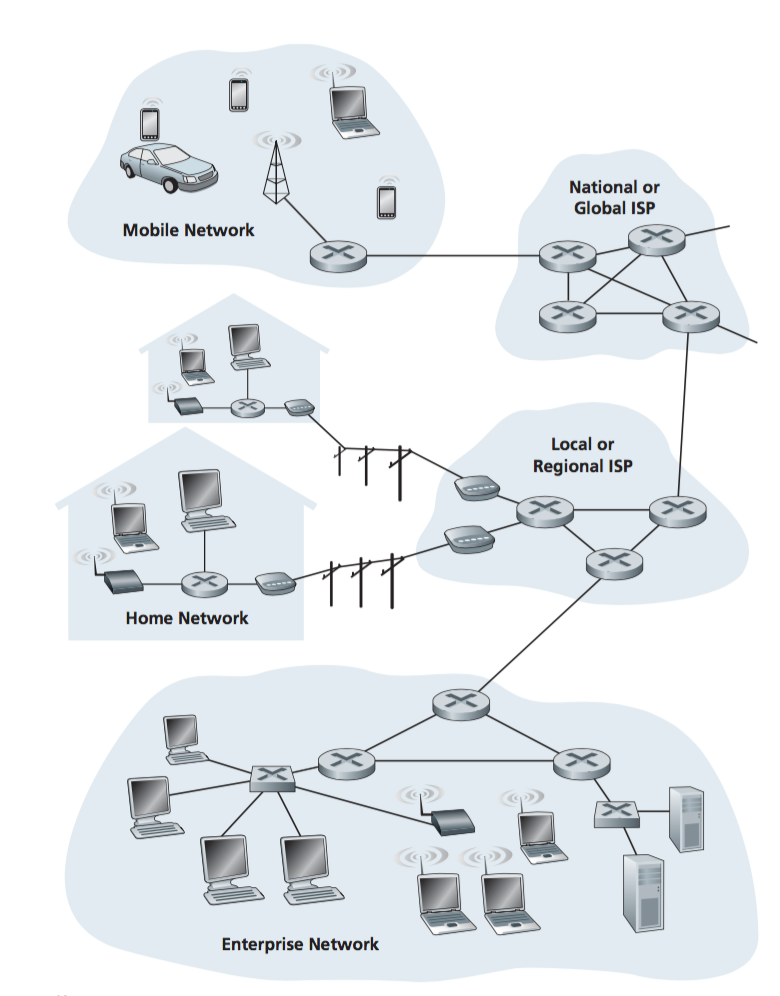
\includegraphics[scale=0.5]{1-networks/internet.png}

\subsection{Home access}
\begin{itemize}
	\item DSL (Digital Subscriber Line)
	\item Cable
	\item FTTH (Fiber To The Home)
	\item Dial-up
	\item Satelite
\end{itemize}

\subsection{Packet switching}
\begin{itemize}
	\item Store-and-forward transmission
	\item Output buffer for hver link
	\item Forwarding table
	\item Queing delays
\end{itemize}

\subsection{Circuit switching}
\begin{itemize}
	\item Reserverer en rute til destinationen (end-to-end)
	\item Ingen delays
\end{itemize}

{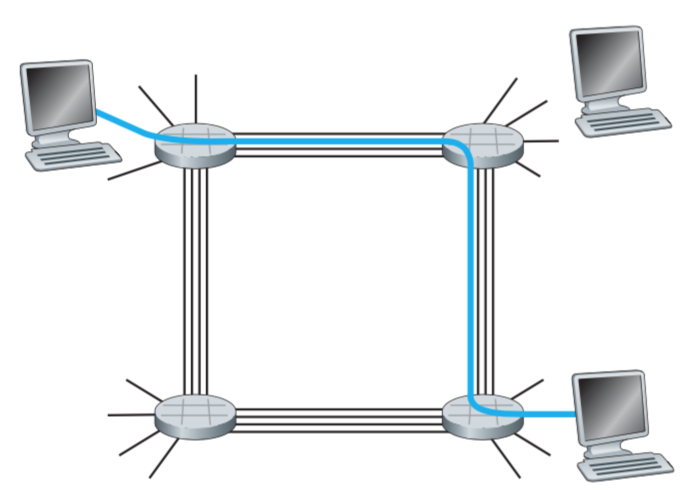
\includegraphics[scale=0.7]{1-networks/circuit-switched-network.png}

\section{Protokol}

\subsection{Hvad er en protokol}
\begin{itemize}
	\item Regelsæt
	\item Definerer måden hvorpå en opgave skal udføres
\end{itemize}

\subsection{Hvad bruger vi protokoller til?}
\begin{itemize}
	\item At have en fælles bestemmelse for hvordan 2 systemer/entiteter kommunikerer, uden de har kendskab til hinandens indre virkener
	\item Mindsker fejlmargin
\end{itemize}

{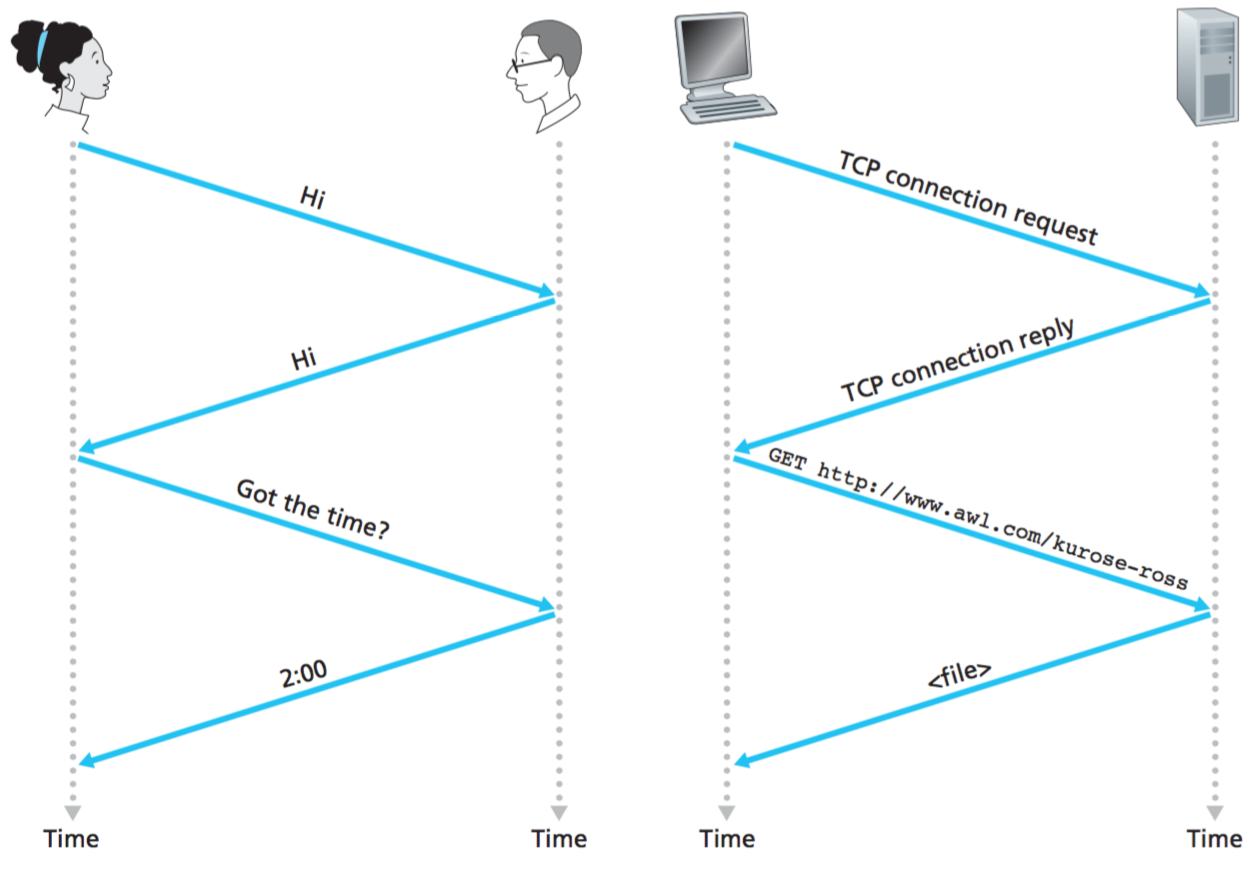
\includegraphics[scale=0.7]{1-networks/protokol.png}

\subsection{Protokoller}
\begin{itemize}
	\item IP
	\item TCP
	\item UDP
	\item HTTP(S)
	\item FTP(S)
	\item SMTP
	\item ...
\end{itemize}

\section{Netværkslag}

\subsection{Modeller}
\begin{itemize}
	\item Fem-lags internet protokol stack
	\item Syv-lags ISO (International Standards Organization) OSI (Open Systems Interconnection) model
\end{itemize}

{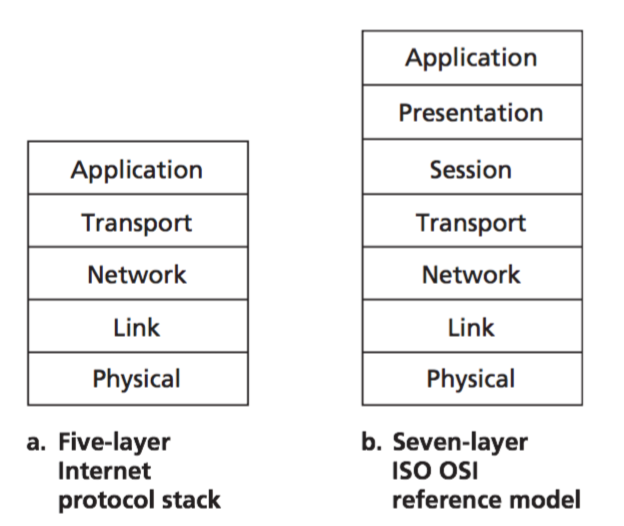
\includegraphics[scale=1]{1-networks/netvaerkslag.png}